% Final submitted source. Repository asset paths are used; visual output matches the submitted PDF.
\documentclass[11pt,a4paper]{article}

\usepackage[margin=25mm,headsep=7mm,footskip=12mm]{geometry}
\usepackage{fontspec}
\usepackage{xeCJK}
\setmainfont{Noto Serif}
\setsansfont{Noto Sans}
\setmonofont{Noto Sans Mono CJK JP}[Scale=0.90]
\setCJKmainfont{Noto Serif CJK JP}
\setCJKsansfont{Noto Sans CJK JP}
\setCJKmonofont{Noto Sans Mono CJK JP}[Scale=0.90]
\XeTeXlinebreaklocale "ja"
\XeTeXlinebreakskip=0pt plus 1pt
\xeCJKsetup{CJKecglue=\hskip 0.12em plus 0.08em minus 0.04em}

\usepackage{amsmath,amssymb,bm}
\usepackage{graphicx}
\usepackage{booktabs,tabularx,array,longtable,makecell,adjustbox}
\usepackage{caption}
\usepackage{float}
\usepackage{placeins}
\usepackage{enumitem}
\usepackage{listings}
\usepackage{xcolor}
\usepackage{etoolbox}
\usepackage{fancyhdr}
\usepackage{titlesec}
\usepackage{setspace}
\usepackage[hidelinks]{hyperref}
\patchcmd{\thebibliography}{\section*{\refname}}{}{}{}

\setstretch{1.04}
\setlength{\parindent}{1em}
\setlength{\parskip}{0pt}
\setlength{\emergencystretch}{2em}
\raggedbottom

\definecolor{HeadingBlue}{HTML}{1F3A5F}
\definecolor{RuleGray}{HTML}{9AA5B1}
\definecolor{CodeBg}{HTML}{F5F7FA}
\definecolor{CodeRule}{HTML}{CBD5E0}

\titleformat{\section}
  {\sffamily\bfseries\Large\color{HeadingBlue}}
  {\thesection}{0.8em}{}
  [\vspace{0.2em}\color{RuleGray}\titlerule]
\titlespacing*{\section}{0pt}{2.0em}{0.9em}
\titleformat{\subsection}
  {\sffamily\bfseries\large\color{HeadingBlue}}
  {\thesubsection}{0.7em}{}
\titlespacing*{\subsection}{0pt}{1.4em}{0.55em}

\captionsetup{font=small,labelfont=bf,labelsep=quad,justification=centering}
\renewcommand{\figurename}{図}
\renewcommand{\tablename}{表}

\pagestyle{fancy}
\fancyhf{}
\fancyhead[L]{\small 2026年度 シミュレーション工学・演習 最終課題}
\fancyfoot[C]{\small\thepage}
\renewcommand{\headrulewidth}{0.3pt}
\setlength{\headheight}{14pt}

\lstdefinelanguage{Matlab}{
  keywords={function,end,if,elseif,else,for,while,return,true,false},
  sensitive=true,
  morecomment=[l]{\%},
  morestring=[b]"
}
\lstset{
  language=Matlab,
  basicstyle=\ttfamily\footnotesize,
  keywordstyle=\bfseries,
  commentstyle=\color{gray},
  numbers=left,
  numberstyle=\scriptsize,
  numbersep=7pt,
  frame=single,
  rulecolor=\color{CodeRule},
  backgroundcolor=\color{CodeBg},
  breaklines=true,
  breakatwhitespace=false,
  columns=fullflexible,
  keepspaces=true,
  showstringspaces=false,
  tabsize=2,
  xleftmargin=1.7em,
  framexleftmargin=1.2em,
  aboveskip=0.8em,
  belowskip=0.8em
}

\newcommand{\code}[1]{\texttt{#1}}
\newcommand{\vect}[1]{\bm{#1}}
\newcommand{\RMSE}{\mathrm{RMSE}}

\begin{document}

\begin{titlepage}
\thispagestyle{empty}
\centering
\vspace*{24mm}
{\sffamily\Large 2026年度\par}
\vspace{5mm}
{\sffamily\bfseries\LARGE シミュレーション工学・演習　最終課題\par}
\vspace{18mm}
{\color{HeadingBlue}\rule{0.82\textwidth}{0.8pt}\par}
\vspace{14mm}
{\sffamily\bfseries\fontsize{21pt}{30pt}\selectfont
遠隔操作ロボットの通信遅延に対する\par
定速度予測補償の有効範囲\par}
\vspace{8mm}
{\large 一次遅れ・純遅延モデルを用いた軌道追従解析\par}
\vspace{14mm}
{\color{HeadingBlue}\rule{0.82\textwidth}{0.8pt}\par}
\vfill
\renewcommand{\arraystretch}{1.5}
\begin{tabular}{>{\sffamily\bfseries}r l}
学年・組 & 4年7組 \\
番号 & 106番 \\
氏名 & 三ツ井雅翔
\end{tabular}
\vspace{22mm}
\end{titlepage}

\setcounter{page}{1}

\section{シミュレーションの目的}

遠隔操作ロボットでは、操作者が生成した指令を通信回線を介してロボットへ送るため、指令が生成されてから利用可能になるまでに通信遅延が生じる。さらに、指令を一定周期で送信する場合、受信側が使用する最新指令はサンプル間でも古くなる。古い位置指令をそのまま保持するゼロ次ホールド（Zero-Order Hold、以下 ZOH）は実装が容易である一方、目標運動が速いほど位置の遅れが大きくなる。

通信遅延が遠隔操作性能を低下させることは古くから報告されており、Sheridanらは伝送遅延を含む遠隔マニピュレーションで作業時間が増加することを示した\cite{sheridan1963}。遅延の影響を軽減する方法として、実ロボットより先に動く仮想ロボットを表示する予測表示\cite{bejczy1990}、遠隔側の詳細な動力学モデルを必須としない予測器フレームワーク\cite{zheng2018,zheng2020}、操作者の意図軌道を予測して車両を誘導する方式\cite{zhang2023}などが研究されている。

本課題が想定するのは、遠隔地の操作者がロボット手先の目標位置を生成し、その位置と速度を一定周期でロボット側へ送信する場面である。対象動作は、接触を伴わない2次元平面内の自由空間運動とする。人間の操作過程そのものはモデル化せず、操作者が生成する理想的な手先位置指令を、再現可能な円軌道と1:2リサジュー軌道で代用する。したがって、本課題が評価するのは、人間、映像フィードバックおよび力覚を含む遠隔操作系全体ではなく、片方向の位置指令伝送と受信側の指令再構成が手先追従誤差へ与える影響である。

本課題では、複雑な予測器や人間操作者を含む実験に進む前の基礎検討として、最後に受信した目標位置と目標速度から、現在時刻の目標位置指令を一次外挿する定速度予測（Constant Velocity、以下 CV）を扱う。本稿のCVはロボットの実状態を予測するものではなく、送信側で生成された目標指令を受信側で前方外挿する単純なデッドレコニングである。このため、予測表示\cite{bejczy1990}、Zhengらの予測器フレームワーク\cite{zheng2018,zheng2020}、予測軌道誘導制御\cite{zhang2023}と同一の方式ではない。

この対象を選んだ理由は、通信遅延が遠隔操作ロボットの基本的な性能制約であり、単純な予測補償でも有効条件と失敗条件の双方を数値的に検討できるためである。本シミュレーションの目的は、通信遅延、目標軌道の角周波数および軌道形状を変化させ、CVがZOHより追従誤差を低減する条件と、定速度仮定の破綻によって逆に悪化する条件を明らかにすることである。特に、遅延時間を軌道の時間スケールで無次元化し、改善から悪化へ移る範囲を整理する。本課題の着眼点は、CVが有効かどうかだけでなく、単純な外挿がZOHより悪化する条件を、離散条件格子と無次元量の両面から明示することにある。

\section{関連研究}

Sheridanら\cite{sheridan1963}は、遠隔マニピュレータを用いた単純作業に伝送遅延を導入し、遅延が人間の操作時間へ与える影響を調べた。この研究は、通信遅延が単なる信号処理上の問題ではなく、人間を含む遠隔操作全体の性能を低下させることを示した初期の研究である。

Bejczyら\cite{bejczy1990}は、実ロボットの遅延映像へリアルタイムの仮想ロボットを重ねる phantom robot を提案し、長い遅延を含む自由空間動作で予測表示が作業性能を改善し得ることを報告した。ただし、これは操作者へ将来のロボット状態を提示する方式であり、本課題のようにロボットへ送る位置指令自体を外挿する方式とは異なる。

Zhengら\cite{zheng2018}は、遠隔サブシステムの詳細な動的モデルを必要としない予測器フレームワークをネットワーク化閉ループ系へ適用し、一定遅延だけでなく変動遅延へ拡張した。さらに高速度無人地上車両の human-in-the-loop 実験では、予測器を用いることで走行速度、横方向追従精度および操舵努力が改善したと報告している\cite{zheng2020}。これらは、予測により遅延の負の影響を軽減できる実例である一方、予測器の構造と評価対象は本課題の一次 Taylor 外挿とは異なる。

Zhangら\cite{zhang2023}は、操作者の意図軌道を予測し、車両をその軌道へ誘導する PTGC（Predicted Trajectory Guidance Control）を提案した。同研究では、実験条件において大きな遅延では操縦性を改善した一方、小さな遅延では効果が限定的であった。本課題では、人間の適応や認知負荷を扱わず、同じ通信条件とロボット側の局所位置応答条件の下で、ZOHとCVの数値誤差だけを比較する。この限定により、定速度外挿の有効範囲を再現可能な条件で調べる。

\section{遠隔位置指令系のモデル化}

\subsection{対象システム}

本課題では、操作者が遠隔地からロボット手先の目標位置を指令し、ネットワークを介してその指令をロボット側へ送る状況を想定する。送信する量は関節角、力、トルクではなく、2次元平面内の手先目標位置とその目標速度である。対象動作は障害物や物体との接触を含まない自由空間の軌道追従とし、人間の操作入力は解析的な試験軌道で代用する。

ロボット側には、受信した手先位置指令へ追従する局所位置制御系が既に存在すると仮定する。本課題における制御対象の出力はロボット手先位置 $\vect x(t)$、入力は受信側で再構成された手先位置指令 $\vect u(t)$ である。局所位置制御器、アクチュエータおよび機械応答を個別にはモデル化せず、指令位置から実際の手先位置までの閉ループ応答を、各軸独立の一次遅れ系として近似する。本課題では局所位置制御器そのものの設計や安定性解析は行わず、安定な局所位置制御系が既に構成されていることを前提として、通信後の位置指令再構成方式だけを比較する。

したがって、解析範囲は「操作者が生成した位置指令が通信され、受信側で再構成され、ロボット手先が追従するまで」である。映像や状態の操作者側への返送、人間の認知・適応、逆運動学、関節制限、接触、力覚および安全制約は対象外とする。これにより、通信遅延と指令再構成方式の差を分離して評価する。

本稿で用いる主な記号を表\ref{tab:symbols}に示す。

\begin{table}[H]
\centering
\caption{主な記号と単位}
\label{tab:symbols}
\begin{tabular}{clc}
\toprule
記号 & 意味 & 単位 \\
\midrule
$t$ & 現在時刻 & s \\
$t_k$ & パケット送信時刻 & s \\
$h_s$ & 送信周期 & s \\
$L$ & 片道通信遅延 & s \\
$a(t)$ & 使用中のパケット齢 & s \\
$\vect r(t)$ & 操作者が生成する理想手先位置指令 & m \\
$\vect u(t)$ & 受信側で再構成した手先位置指令 & m \\
$\vect x(t)$ & ロボット手先位置 & m \\
$T$ & 局所位置応答の時定数 & s \\
$A$ & 軌道振幅 & m \\
$\omega$ & 基本角周波数 & rad/s \\
$G$ & CVとZOHのRMSE比 & 無次元 \\
\bottomrule
\end{tabular}
\end{table}

\begin{figure}[H]
\centering
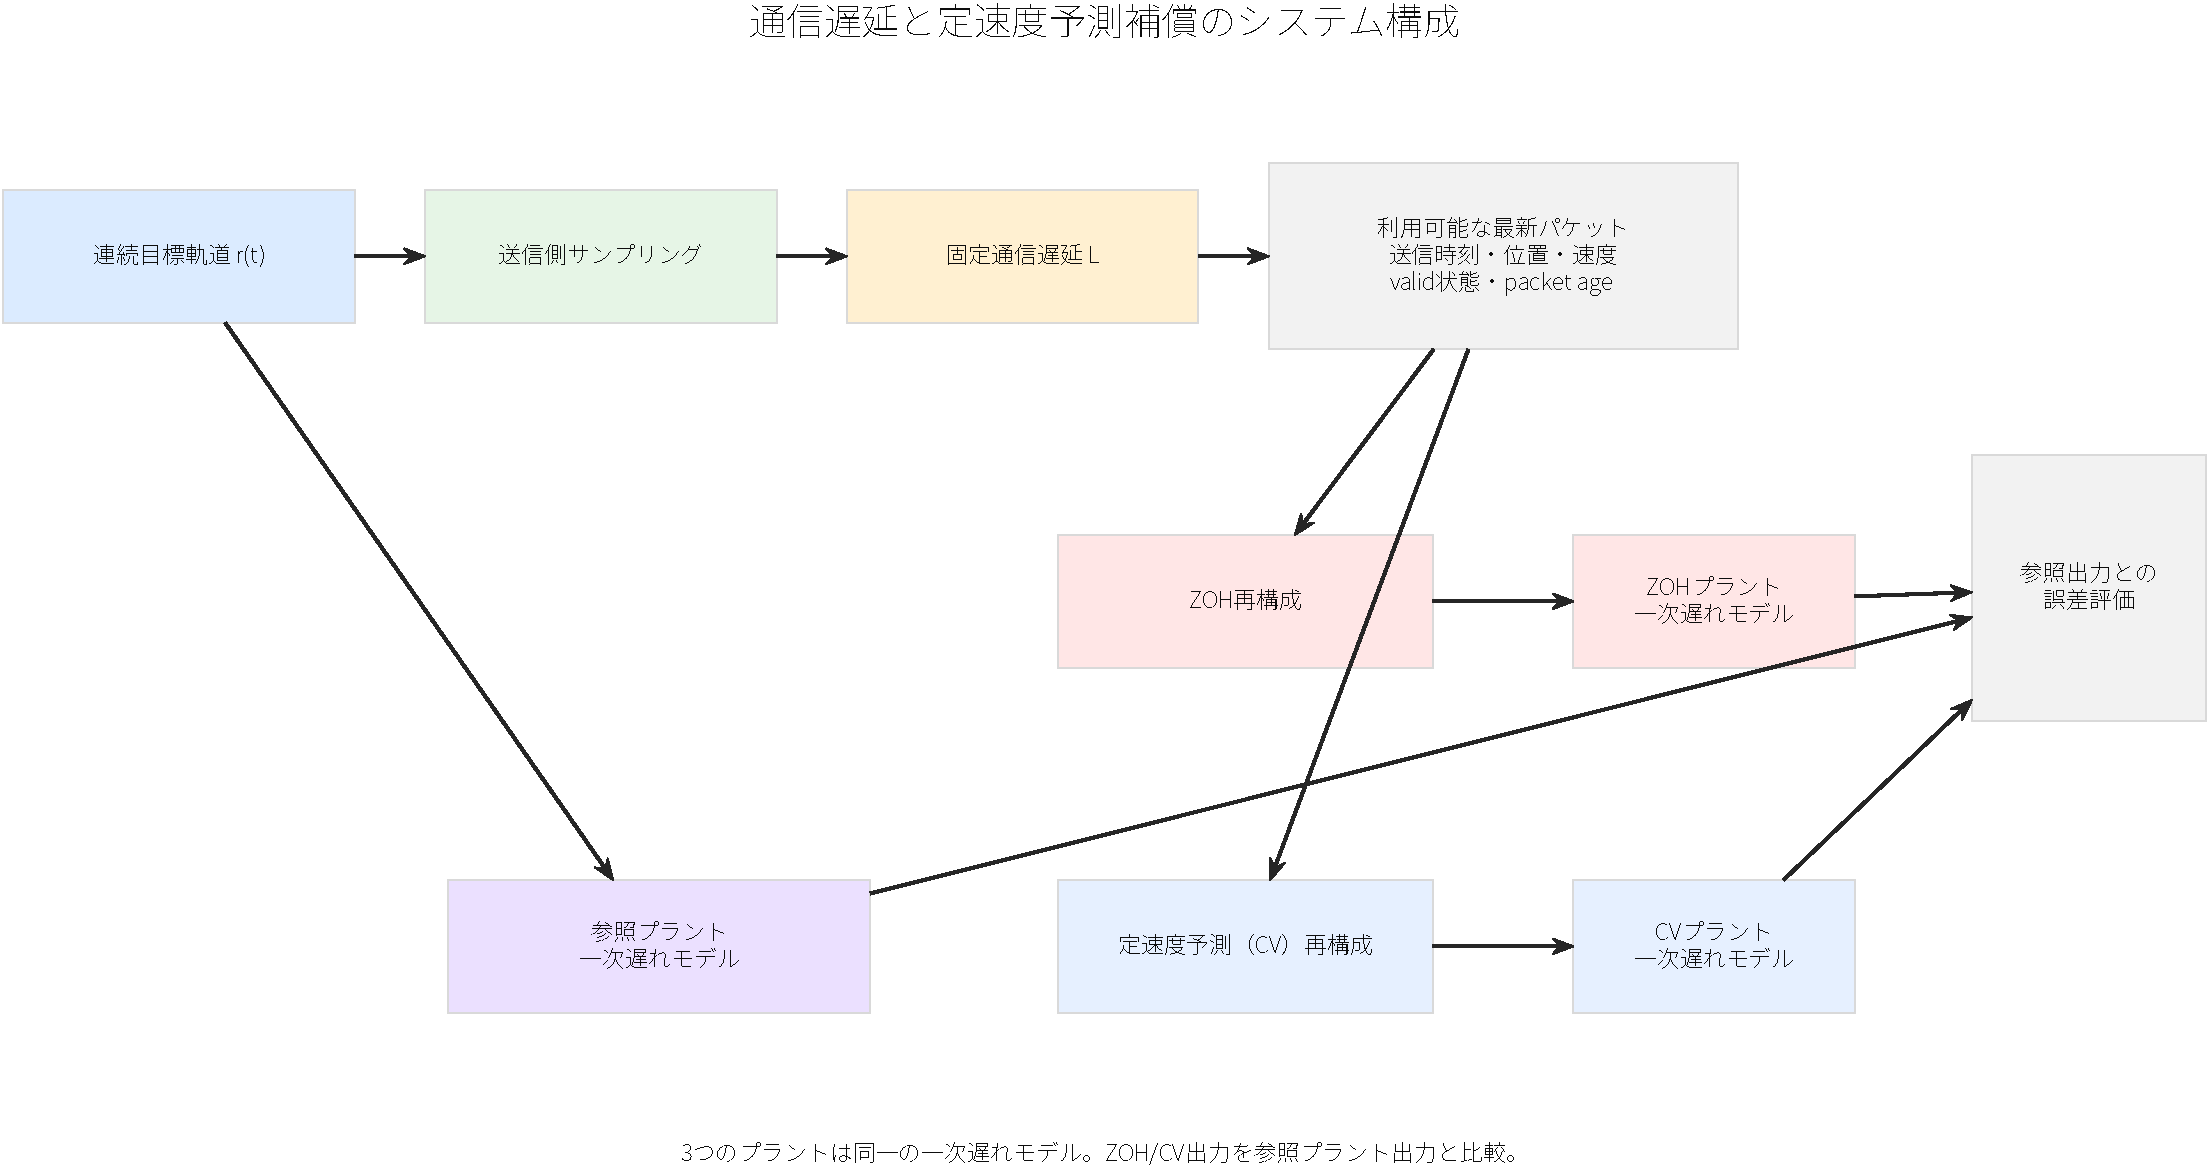
\includegraphics[width=0.98\linewidth]{../assets/issue9/figures/figure_01_system_architecture.pdf}
\caption{想定する片方向遠隔位置指令系と比較経路}
\label{fig:system}
\end{figure}

図\ref{fig:system}に示すように、操作者入力を代用する理想手先軌道は、通信経路と遅延なし基準経路に分岐する。通信経路では、送信側サンプリング、固定通信遅延、最新パケット選択を経て、ZOHまたはCVにより現在時刻の位置指令を再構成する。図中の「局所位置応答」は、ロボット側の局所位置制御器、アクチュエータおよび機械応答をまとめた一次遅れ近似を表す。

通信経路では、送信側で目標位置と目標速度をサンプリングし、固定通信遅延後に利用可能となった最新パケットからZOH指令とCV指令を生成する。遅延なし基準経路では、同じ理想手先位置指令を通信を介さず、同じ局所位置応答モデルへ直接入力する。3経路で同一の応答モデルを使うことで、ロボット側の応答遅れを共通化し、通信と指令再構成によって追加される誤差だけを比較する。

\subsection{送信パケットと利用可能条件}

送信周期を $h_s$ とし、送信時刻を
\begin{equation}
 t_k = k h_s
\end{equation}
とする。各パケットには、送信時刻 $t_k$、目標位置 $\vect r(t_k)$、目標速度 $\dot{\vect r}(t_k)$ を格納する。本シミュレーションでは、目標速度をセンサ計測や位置差分から推定せず、後述する軌道式から解析的に計算した正確な値を位置とともに送信する。一定の片道通信遅延を $L$ とすると、時刻 $t$ で利用できるパケットは
\begin{equation}
 t_k + L \le t
\end{equation}
を満たすものに限られ、その中で最も新しいパケットを使用する。現在時刻と採用したパケットの送信時刻との差をパケット齢 $a(t)$ とし、
\begin{equation}
 a(t)=t-t_k
\end{equation}
と定義する。ここで、$L$ はネットワーク上で固定した伝送遅延であるのに対し、$a(t)$ は現在使用しているパケットが生成されてからの経過時間である。したがって、パケット齢には通信遅延だけでなく、サンプリング後に次のパケットへ更新されるまでの経過時間も含まれ、$L=0$ であっても一般に $a(t)>0$ となる。

\subsection{ZOHとCVによる指令再構成}

ZOHでは、最後に利用可能となった位置を次の更新まで保持する。
\begin{equation}
 \vect u_{\mathrm{ZOH}}(t)=\vect r(t_k)
\end{equation}
CVでは、同じパケットの位置と速度を用い、パケット齢だけ線形外挿する。
\begin{equation}
 \vect u_{\mathrm{CV}}(t)=\vect r(t_k)+a(t)\dot{\vect r}(t_k)
\end{equation}
CVが予測するのはロボットの実際の手先状態ではなく、最後に受信した目標位置と目標速度から推定した現在時刻の目標位置指令である。この点で、ロボットの動的モデルと遅延モデルを用いて閉ループ系を構成する Smith 予測器とは異なる。目標指令が一定速度で変化する区間では現在時刻の指令を正確に再現できるが、加速度や方向変化が大きいほど外挿誤差が増える。

\subsection{ロボット側の局所位置応答モデル}

受信側で再構成された手先位置指令から、実際のロボット手先位置までの応答を、各軸独立かつ同一の一次遅れ系として
\begin{equation}
 T\dot{\vect x}(t)+\vect x(t)=\vect u(t)
\end{equation}
で表す。ここで、$\vect u(t)$ はZOH、CVまたは遅延なし基準経路から与えられる手先位置指令、$\vect x(t)$ はその指令に対するロボット手先位置、$T$ は局所位置応答の時定数である。この一次遅れ系はロボットの機械系だけを意味するものではなく、ロボット側の局所位置制御器、アクチュエータおよび機械応答をまとめた閉ループ近似である。3経路は同じ応答モデル、時定数および初期状態を共有する。

\subsection{目標軌道}

人間操作者の入力を直接記録する代わりに、再現可能で位置・速度・加速度を解析的に求められる2種類の試験軌道を、理想手先位置指令として用いる。軌道振幅を $A$、角周波数を $\omega$ とする。基準となる円軌道は
\begin{equation}
 \vect r_{\mathrm{circle}}(t)=
 \begin{bmatrix}
 A\cos(\omega t)\\
 A\sin(\omega t)
 \end{bmatrix}
\end{equation}
とした。円軌道は単一角周波数を持ち、速度の大きさが一定であるため、位相遅れと無次元量を解釈しやすい。

方向変化と複数の周波数成分を含む軌道として、1:2リサジュー軌道を
\begin{equation}
 \vect r_{\mathrm{Lissajous}}(t)=
 \begin{bmatrix}
 A\sin(\omega t)\\
 A\sin(2\omega t)
 \end{bmatrix}
\end{equation}
とした。$y$方向に $2\omega$ の成分を含むため、基本周波数 $\omega$ だけでは運動の速い変化を表し切れない。

\subsection{評価指標}

評価の基準は理想手先位置指令 $\vect r(t)$ そのものではなく、その指令を通信遅延なしで同じ局所位置応答モデルへ直接入力した出力 $\vect x_{\mathrm{ref}}(t)$ とする。以下、この出力を「遅延なし基準応答」または「参照出力」と呼ぶ。理想指令そのものを基準にすると、ロボット側の局所応答遅れまで通信方式の誤差へ含まれるため、同じ応答モデルを通した基準を用いて通信と指令再構成による追加誤差を評価する。方式 $m\in\{\mathrm{ZOH},\mathrm{CV}\}$ の誤差ベクトルと大きさを
\begin{equation}
 \vect e_m(t_i)=\vect x_m(t_i)-\vect x_{\mathrm{ref}}(t_i),
 \qquad
 e_m(t_i)=\lVert\vect e_m(t_i)\rVert_2
\end{equation}
とし、評価区間の $N$ サンプルからRMSEを
\begin{equation}
 \RMSE_m=\sqrt{\frac{1}{N}\sum_{i=1}^{N}e_m(t_i)^2}
\end{equation}
で求める。CVとZOHの性能比を
\begin{equation}
 G=\frac{\RMSE_{\mathrm{CV}}}{\RMSE_{\mathrm{ZOH}}}
\end{equation}
とする。この定義では、$G<1$ はCVのRMSEがZOHより小さいこと、$G=1$ は両者が同じこと、$G>1$ はCVのRMSEがZOHより大きいことを表す。改善率を
\begin{equation}
 I=(1-G)\times100\ \mathrm{[\%]}
\end{equation}
とする。最大誤差、振幅 $A$ で正規化したNRMSE、評価区間内の平均パケット齢 $\overline a$ も保存する。

数値誤差による境界付近の誤分類を避けるため、4.4節で示す代表5条件の時間刻み収束確認から、本実験専用の数値判定幅を $\delta=0.007883$ と定めた。この値は一般的なCV評価の標準閾値ではない。正式な分類規則を
\begin{equation}
\label{eq:classification-rule}
\begin{cases}
G<1-\delta & : \text{改善},\\
|G-1|\le\delta & : \text{同等},\\
G>1+\delta & : \text{悪化}
\end{cases}
\end{equation}
とした。

\section{シミュレーション条件}

\subsection{仮定と初期条件}

本課題では、固定通信遅延、パケット損失なし、遅延揺らぎなし、順序入替えなしとする。局所位置応答モデルの初期位置は $\vect x(0)=\vect 0$ とし、最初のパケットが到着するまでは通信出力を無効とする。過去のパケットを開始前に事前投入しない。

開始前の架空パケットを事前投入しないため、シミュレーション開始直後には利用できるパケット履歴が不足する。また、局所位置応答モデルの起動過渡も生じる。これらを評価から除外するため、各条件を10周期実行し、最初の2周期をウォームアップとして除外した。シミュレーション終了時刻は10周期を覆う最小の固定時間格子点へ切り上げた。

\subsection{標準実験条件}

\begin{table}[H]
\centering
\caption{標準シミュレーション条件}
\label{tab:conditions}
\begin{tabular}{lr}
\toprule
項目 & 設定値 \\
\midrule
軌道 & 円軌道、1:2リサジュー軌道 \\
軌道振幅 $A$ & 1.0 m \\
角周波数 $\omega$ & 0.5、1.0、2.0、4.0 rad/s \\
通信遅延 $L$ & 0、0.10、0.20、0.40、0.50 s \\
送信周期 $h_s$ & 0.020 s \\
局所位置応答時定数 $T$ & 0.10 s \\
固定時間刻み & 0.005 s \\
数値解法 & 4次 Runge--Kutta 法（Simulink \code{ode4}） \\
総実行時間 & 各角周波数について10周期 \\
評価除外区間 & 最初の2周期 \\
比較方式 & 遅延なし参照、ZOH、CV \\
\bottomrule
\end{tabular}
\end{table}

軌道振幅 $A=1.0\ \mathrm{m}$ は、特定の実機ロボットの作業領域を表す値ではなく、線形モデル上で誤差を比較するための基準スケールとして設定した。本モデルでは位置と追従誤差が振幅に比例する一方、RMSE比 $G$ は原則として振幅に依存しないため、$A=1$ と置くことで結果を読み取りやすくした。送信周期 $h_s=0.020\ \mathrm{s}$ は50 Hzの指令更新に相当する。局所位置応答時定数 $T=0.10\ \mathrm{s}$ は特定実機から同定した値ではなく、通信遅延と比較可能な時間スケールを持つ代表的な一次遅れ応答として設定した。通信遅延 $L$ は無遅延から明確な性能悪化が現れる範囲まで、角周波数 $\omega$ は周期約12.6 sから1.57 sまでを覆う探索範囲として選定した。

2軌道、5遅延、4角周波数の完全要因計画、すなわち $2\times5\times4=40$ 条件を逐次実行した。以下で「全40条件」または「標準40条件」と記す場合は、この組合せを指す。各条件では遅延なし基準、ZOHおよびCVを同一Simulink実行内で計算し、条件差以外の影響を避けた。

\subsection{無次元量}

通信遅延と軌道の時間スケールを比較するため、名目遅延に基づく量と実際のパケット齢に基づく量を
\begin{equation}
 q_L=\omega L,
 \qquad
 q_a=\omega\overline a
\end{equation}
とする。さらに $\omega T$ と $\omega h_s$ も保存した。ただし、本実験では $T$ と $h_s$ を固定したため、両者の独立した影響をこの40条件だけから分離することはできない。

\subsection{数値収束の確認}

全40条件を再計算する代わりに、両軌道について最大改善条件、境界近傍条件および最大悪化条件を含む代表5条件を選び、固定時間刻みを0.005 sから0.0025 sへ半減した。選定条件と性能比の変化を表\ref{tab:convergence}に示す。

\begin{table}[H]
\centering
\caption{代表5条件における時間刻み収束の確認}
\label{tab:convergence}
\scriptsize
\setlength{\tabcolsep}{4.0pt}
\begin{tabular}{llrrrrr}
\toprule
軌道 & 選定理由 & $\omega$ & $L$ & $G_{0.005}$ & $G_{0.0025}$ & $|\Delta G|$ \\
 & & [rad/s] & [s] & & & \\
\midrule
円 & 最大改善 & 0.5 & 0.0 & 0.0032960 & 0.0032886 & 0.0000074 \\
円 & 最大悪化・境界近傍 & 4.0 & 0.5 & 1.0843108 & 1.0853042 & 0.0009934 \\
1:2リサジュー & 最大改善 & 0.5 & 0.0 & 0.0060744 & 0.0060607 & 0.0000137 \\
1:2リサジュー & 境界近傍 & 2.0 & 0.5 & 0.9656461 & 0.9664096 & 0.0007635 \\
1:2リサジュー & 最大悪化 & 4.0 & 0.5 & 2.0661331 & 2.0681038 & 0.0019707 \\
\bottomrule
\end{tabular}
\end{table}

5条件はいずれも時間刻み半減後に改善・悪化の分類が変化せず、最大変化は1:2リサジュー軌道の最大悪化条件における $|\Delta G|=0.0019707$ であった。本実験では、この最大変化に対して保守的な安全幅4を掛け、
\begin{equation}
 \delta=4\max |\Delta G|
 =4\times0.0019707
 =0.0078828\approx0.007883
\end{equation}
と定めた。係数4は一般的な標準ではなく、今回の離散分類で時間刻み誤差による見かけの反転を避けるために採用した本実験固有の安全幅である。

\section{MATLAB/Simulinkプログラム}

\subsection{プログラム構成}

MATLABは、設定値の検証、固定時間格子の生成、試験軌道の生成、実験条件の管理、Simulink実行、評価指標の計算、全条件の集約、保存および図生成を担当する。Simulinkは、通信処理と3つの局所位置応答モデルの時間応答を計算する。

実装は、単一条件を実行する処理、全40条件を逐次実行して保存する処理、保存結果から分類・境界・代表条件・図表を生成する処理の3つに分けた。実装上、全条件を定義した実験条件表を \code{manifest} と呼ぶが、これは軌道、遅延、角周波数などの設定値を列挙したデータ構造を意味する。本節で掲載する \code{run\_standard\_experiment} は、その実験条件表を用いて全40条件を実行する入口関数である。

Simulinkの Model Reference は、モデルの一部を再利用可能なサブモデルとして分離する機能である。本実装では、送信側サンプリング、固定遅延、最新パケット選択、ZOH/CV再構成を通信サブモデルにまとめ、局所位置応答モデルを別のサブモデルとしてZOH、CV、遅延なし基準の3経路で共有した。

\begin{center}
\fcolorbox{CodeRule}{CodeBg}{%
\parbox{0.92\linewidth}{\small
\textbf{掲載コードの位置づけ}\quad
プログラム1、2、4は実装ファイルから主要処理を抜粋し、紙面に合わせてコメント、補助処理、入力検証およびエラー処理の一部を省略・整形したものである。プログラム3は処理の流れを説明するため、実装を簡略化したMATLAB風の擬似コードである。したがって、いずれも掲載部分だけをコピーして単独実行できることを保証しない。再実行には、補助関数、設定データおよびSimulinkモデルなどを含むプロジェクト一式が必要である。
}}
\end{center}

\subsection{処理手順}

標準実験の処理は次のとおりである。
\begin{enumerate}[leftmargin=2.4em,itemsep=0.18em]
\item 標準条件の一覧を生成し、設定値を検証する。
\item 軌道、通信遅延、角周波数の全組合せについて処理を繰り返す。
\item 固定時間格子と解析軌道を生成する。
\item Simulinkへの入力を作成する。
\item 参照系、ZOH系、CV系を同一条件で実行する。
\item ウォームアップ後の評価区間を抽出する。
\item RMSE、最大誤差、性能比、改善率、平均パケット齢を計算する。
\item 軌道、通信遅延、角周波数などの条件値と結果を保存する。
\item 全40条件を集約し、CSVとMATへ保存する。
\item 保存結果を再読込して整合性を検証する。
\item 代表条件、性能境界、無次元量の図表を生成する。
\end{enumerate}

結果ファイルには、軌道種別、角周波数、通信遅延、送信周期、時定数、時系列および評価指標を同じ行・構造体に保存した。したがって、図表に示した各点は、PDF中に明示した軌道、$\omega$、$L$ の組合せから対応する計算条件へ戻ることができる。

\subsection{Main Program}

以下では、課題のプログラム掲載形式に合わせ、実験全体の入口となる処理をMain Program、そこから呼び出される軌道生成や評価計算をSub Programと呼ぶ。標準40条件を実行するMain Programの主要部をプログラム1に示す。実験条件の作成と検証はSub Programへ分離し、Main Programは保存先の設定と実験実行だけを担当する。

\noindent\textbf{プログラム1　標準40条件を実行するMain Program（実装抜粋）}
\begin{lstlisting}
% Report excerpt; not standalone.
function result = run_standard_experiment(varargin)
projectRoot = fileparts(mfilename("fullpath"));
sourceDirectory = fullfile(projectRoot, "src");
pathBefore = path;
directoryBefore = pwd;
cleanupPath = onCleanup(@() path(pathBefore));
cleanupDirectory = onCleanup(@() cd(directoryBefore));
addpath(sourceDirectory);

parser = inputParser;
addParameter(parser, "OutputRoot", ...
    fullfile(projectRoot, "results", "generated"));
addParameter(parser, "SaveResults", true, ...
    @(value) islogical(value) && isscalar(value));
parse(parser, varargin{:});

manifest = teleopdelay.experiment.standard_manifest();
result = teleopdelay.experiment.run_manifest( ...
    manifest, projectRoot, ...
    "OutputRoot", parser.Results.OutputRoot, ...
    "SaveResults", parser.Results.SaveResults);
clear cleanupDirectory cleanupPath;
end
\end{lstlisting}

\subsection{Sub Programs}

軌道生成は解析式を直接実装し、位置、速度、加速度を同じ時間格子上で返す。円軌道生成の主要部をプログラム2に示す。

\noindent\textbf{プログラム2　円軌道の位置・速度・加速度生成（実装抜粋）}
\begin{lstlisting}
% Report excerpt; inputs are prepared elsewhere.
A = parameters.amplitude;
omega = parameters.omega;
position_m = [ ...
    A * cos(omega * time_s), ...
    A * sin(omega * time_s)];
velocity_mps = [ ...
    -A * omega * sin(omega * time_s), ...
     A * omega * cos(omega * time_s)];
acceleration_mps2 = [ ...
    -A * omega^2 * cos(omega * time_s), ...
    -A * omega^2 * sin(omega * time_s)];
\end{lstlisting}

通信サブモデルで行う最新パケット選択とZOH/CV再構成の要点を、MATLAB風の表記でプログラム3に示す。これは処理の目的と分岐を説明するための読者向け擬似コードであり、実装ファイルと変数名や記述を逐語的に一致させたものではない。特に、最初のパケットが到着する前は有効な指令を出力しないことを明示している。

\noindent\textbf{プログラム3　最新パケット選択とZOH/CV指令再構成（説明用擬似コード）}
\begin{lstlisting}
% Explanatory pseudocode; not verbatim implementation.
available = send_time_s + delay_s <= current_time_s;
latest = find(available, 1, "last");

if isempty(latest)
    packet_valid = false;
    return;
end

packet_valid = true;
packet_age_s = current_time_s - send_time_s(latest);
zoh_command_xy_m = position_xy_m(latest, :);
cv_command_xy_m = position_xy_m(latest, :) ...
    + packet_age_s * velocity_xy_mps(latest, :);
\end{lstlisting}

評価指標は、ウォームアップ後のサンプルだけを選ぶ論理配列 \code{mask} を用い、参照出力との差を同じ評価区間で計算する。RMSE、最大誤差、性能比および改善率の主要部をプログラム4に示す。

\noindent\textbf{プログラム4　追従誤差と性能比の計算（実装抜粋）}
\begin{lstlisting}
% Report excerpt; simulation and mask are prepared elsewhere.
evaluation_packet_age = simulation.packet_age_s(mask);
reference = simulation.reference_position_xy_m;
zoh_error = simulation.zoh_position_xy_m - reference;
cv_error = simulation.cv_position_xy_m - reference;

zoh_error_norm = sqrt(sum(zoh_error.^2, 2));
cv_error_norm = sqrt(sum(cv_error.^2, 2));
rmse_zoh_m = sqrt(mean(sum(zoh_error(mask,:).^2, 2)));
rmse_cv_m = sqrt(mean(sum(cv_error(mask,:).^2, 2)));
max_error_zoh_m = max(zoh_error_norm(mask));
max_error_cv_m = max(cv_error_norm(mask));

zero_tolerance_m = 32 * eps( ...
    max([1; abs(rmse_zoh_m); abs(rmse_cv_m)]));
zoh_is_zero = rmse_zoh_m <= zero_tolerance_m;
cv_is_zero = rmse_cv_m <= zero_tolerance_m;
if zoh_is_zero && cv_is_zero
    performance_ratio = 1.0;
    improvement_percent = 0.0;
elseif zoh_is_zero
    error("teleopDelay:UndefinedPerformanceRatio", ...
        "performance_ratio is undefined when only the ZOH RMSE is zero.");
else
    performance_ratio = rmse_cv_m / rmse_zoh_m;
    improvement_percent = (1.0 - performance_ratio) * 100.0;
end
mean_packet_age_s = mean(evaluation_packet_age);
\end{lstlisting}

掲載したコードは、処理内容を説明するために主要部分だけを抜粋または簡略化したものであり、完全な実装ファイルの代替ではない。実装では、入力配列の形状、時刻整合、パケット有効性、零除算、非有限値および保存結果の整合性を検証し、不正な条件を黙って評価しない。

\section{実行結果}

\subsection{全40条件の分類}

性能比 $G$ と数値収束から定めた本実験専用の許容幅0.007883を用いて分類した結果を表\ref{tab:classification}に示す。ここで、$G<1$ はCV優位、$G>1$ はZOH優位を意味する。

\begin{table}[H]
\centering
\caption{CVによる改善・同等・悪化の条件数}
\label{tab:classification}
\begin{tabular}{lrrrr}
\toprule
軌道 & 改善 & 同等 & 悪化 & 合計 \\
\midrule
円軌道 & 19 & 0 & 1 & 20 \\
1:2リサジュー軌道 & 18 & 0 & 2 & 20 \\
合計 & 37 & 0 & 3 & 40 \\
\bottomrule
\end{tabular}
\end{table}

40条件中37条件でCVのRMSEがZOHより小さくなった。一方、悪化した3条件は高角周波数・大遅延側に集中した。円軌道では $\omega=4\ \mathrm{rad/s},\ L=0.5\ \mathrm{s}$ の1条件、リサジュー軌道では $\omega=4\ \mathrm{rad/s},\ L=0.4,0.5\ \mathrm{s}$ の2条件で悪化した。

\subsection{代表条件の軌跡}

\begin{figure}[H]
\centering
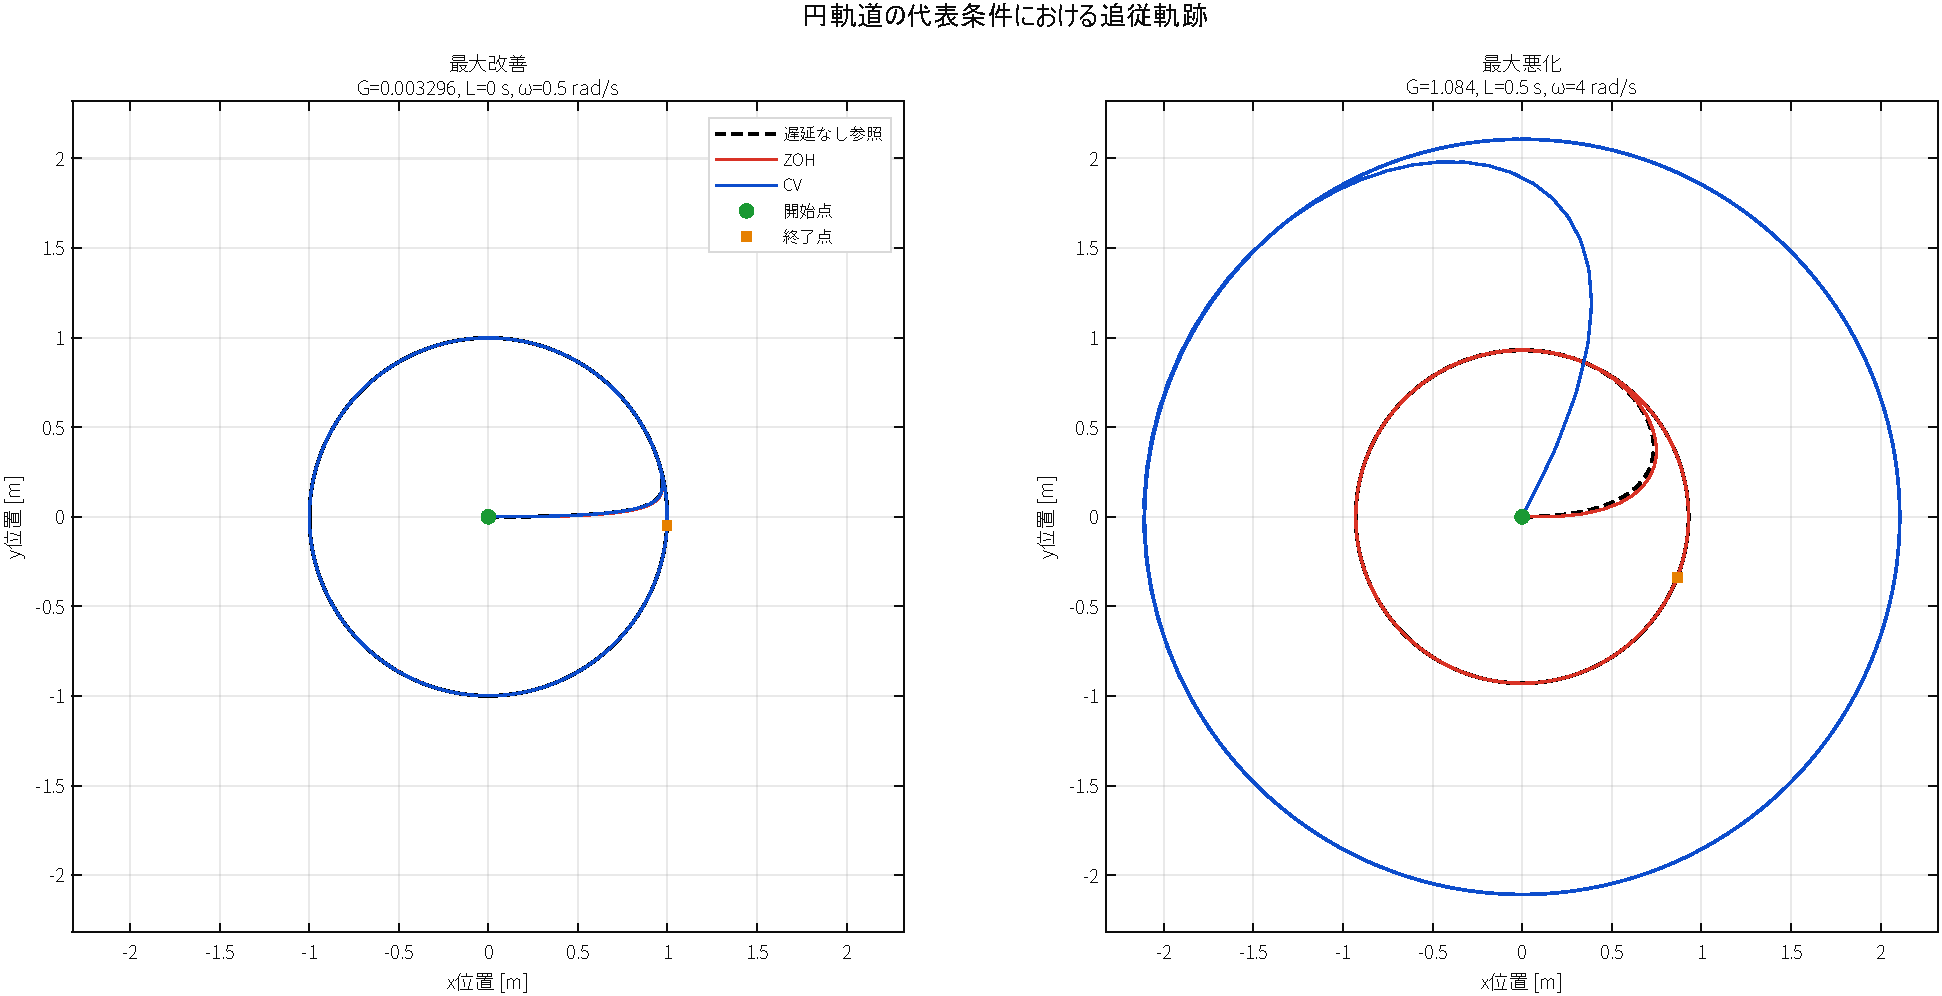
\includegraphics[width=\linewidth]{../assets/issue9/figures/figure_02_representative_circle.pdf}
\caption{円軌道の代表条件における追従軌跡}
\label{fig:circle}
\end{figure}

円軌道の最大改善条件は $\omega=0.5\ \mathrm{rad/s},\ L=0\ \mathrm{s}$ であり、$G=0.00330$、改善率99.67\%であった。最大悪化条件かつ境界最近傍条件は $\omega=4\ \mathrm{rad/s},\ L=0.5\ \mathrm{s}$ であり、$G=1.084$、改善率は$-8.43$\%であった。図\ref{fig:circle}では、低速条件でCVが参照軌道にほぼ一致する一方、高速・大遅延条件ではCVの外挿が参照から外れることが確認できる。

\begin{figure}[H]
\centering
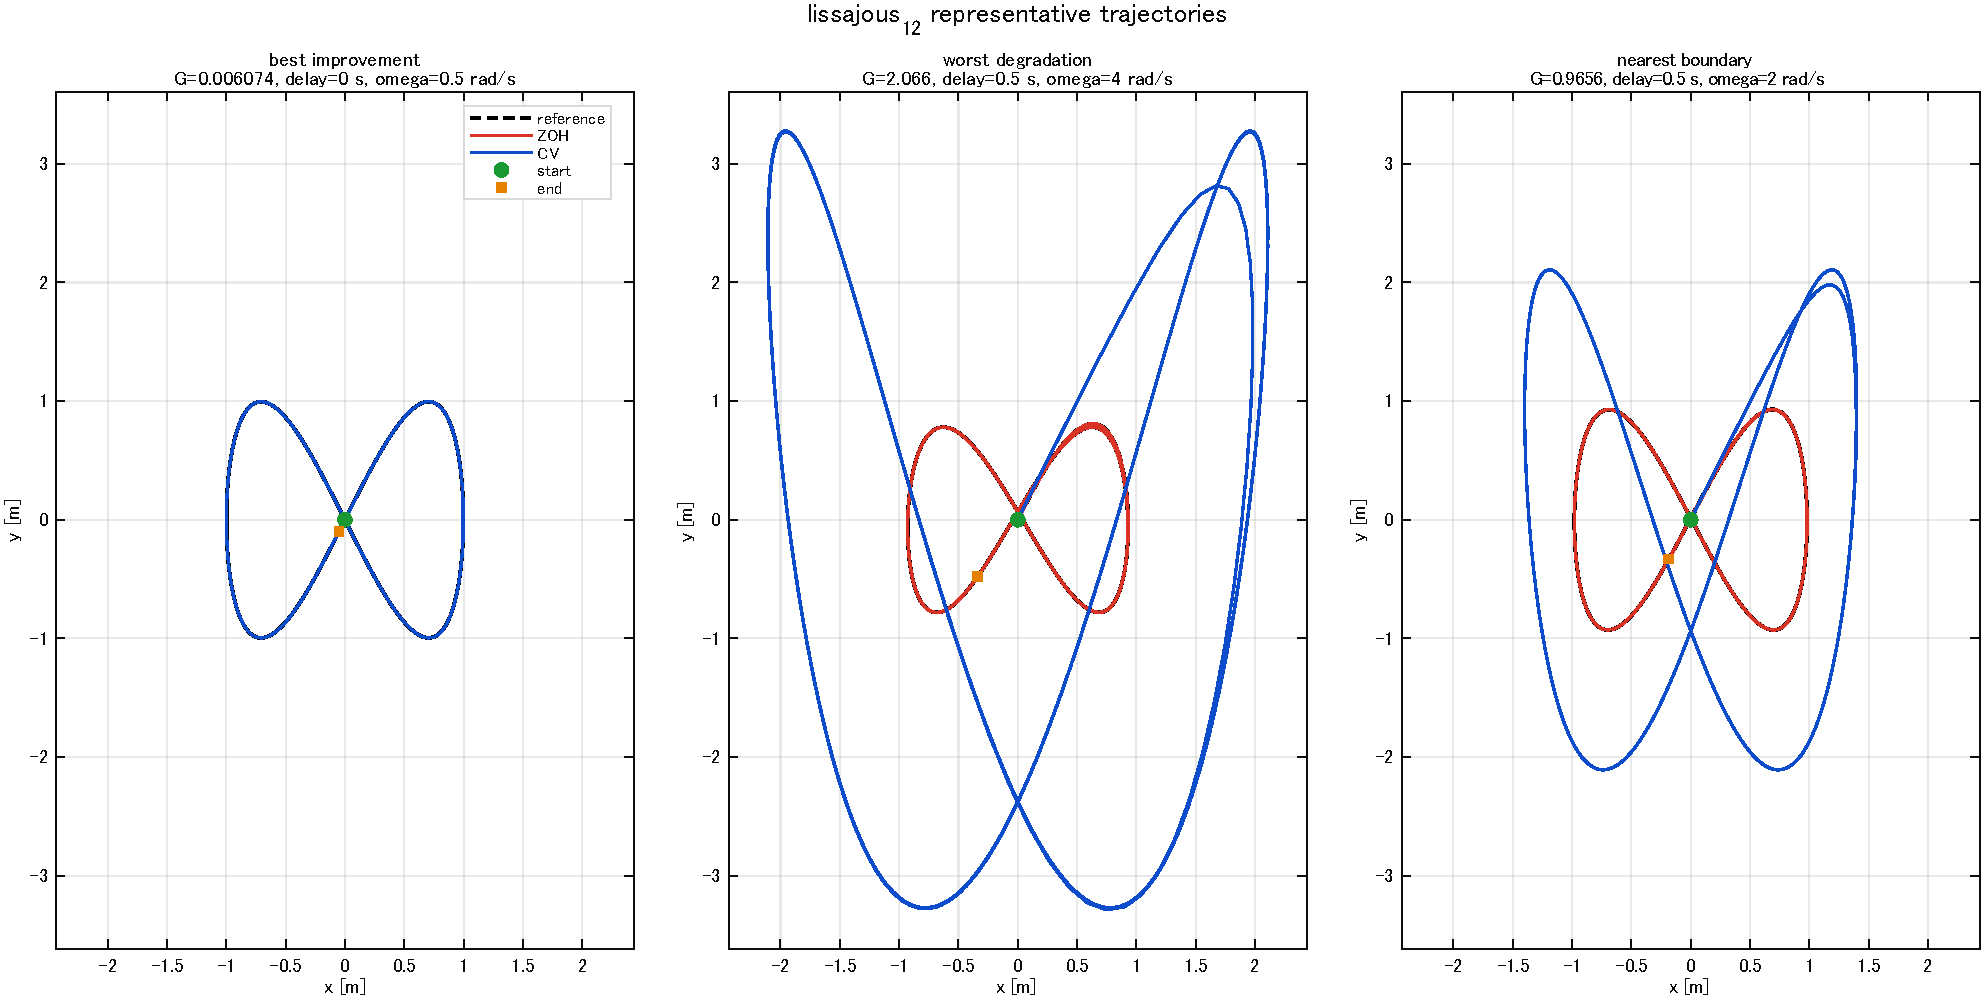
\includegraphics[width=\linewidth]{../assets/issue9/figures/figure_03_representative_lissajous.pdf}
\caption{1:2リサジュー軌道の代表条件における追従軌跡}
\label{fig:lissajous}
\end{figure}

リサジュー軌道の最大改善条件は $\omega=0.5\ \mathrm{rad/s},\ L=0\ \mathrm{s}$ であり、$G=0.00607$、改善率99.39\%であった。境界最近傍条件は $\omega=2\ \mathrm{rad/s},\ L=0.5\ \mathrm{s}$ で $G=0.966$、最大悪化条件は $\omega=4\ \mathrm{rad/s},\ L=0.5\ \mathrm{s}$ で $G=2.066$ であった。最大悪化条件ではCVのRMSEがZOHの約2.07倍になった。

\begin{table}[H]
\centering
\caption{自動選定した主要条件の評価値}
\label{tab:representative}
\scriptsize
\setlength{\tabcolsep}{3.5pt}
\begin{tabular}{llrrrrrr}
\toprule
軌道 & 役割 & $\omega$ & $L$ & RMSE ZOH & RMSE CV & $G$ & 改善率 \\
 & & [rad/s] & [s] & [m] & [m] & & [\%] \\
\midrule
円 & 最大改善 & 0.5 & 0 & 0.004578 & 0.0000151 & 0.00330 & 99.67 \\
円 & \makecell[l]{最大悪化・\\境界最近傍} & 4 & 0.5 & 1.580 & 1.714 & 1.084 & $-8.43$ \\
1:2リサジュー & 最大改善 & 0.5 & 0 & 0.007217 & 0.0000438 & 0.00607 & 99.39 \\
1:2リサジュー & 境界最近傍 & 2 & 0.5 & 1.306 & 1.261 & 0.9656 & 3.44 \\
1:2リサジュー & 最大悪化 & 4 & 0.5 & 1.490 & 3.079 & 2.066 & $-106.61$ \\
\bottomrule
\end{tabular}
\end{table}

負の改善率は悪化を表す。例えば $-106.61$\% は、CVのRMSEがZOHより106.61\%増加したことを示す。

\subsection{誤差時系列と目標加速度}

\begin{figure}[H]
\centering
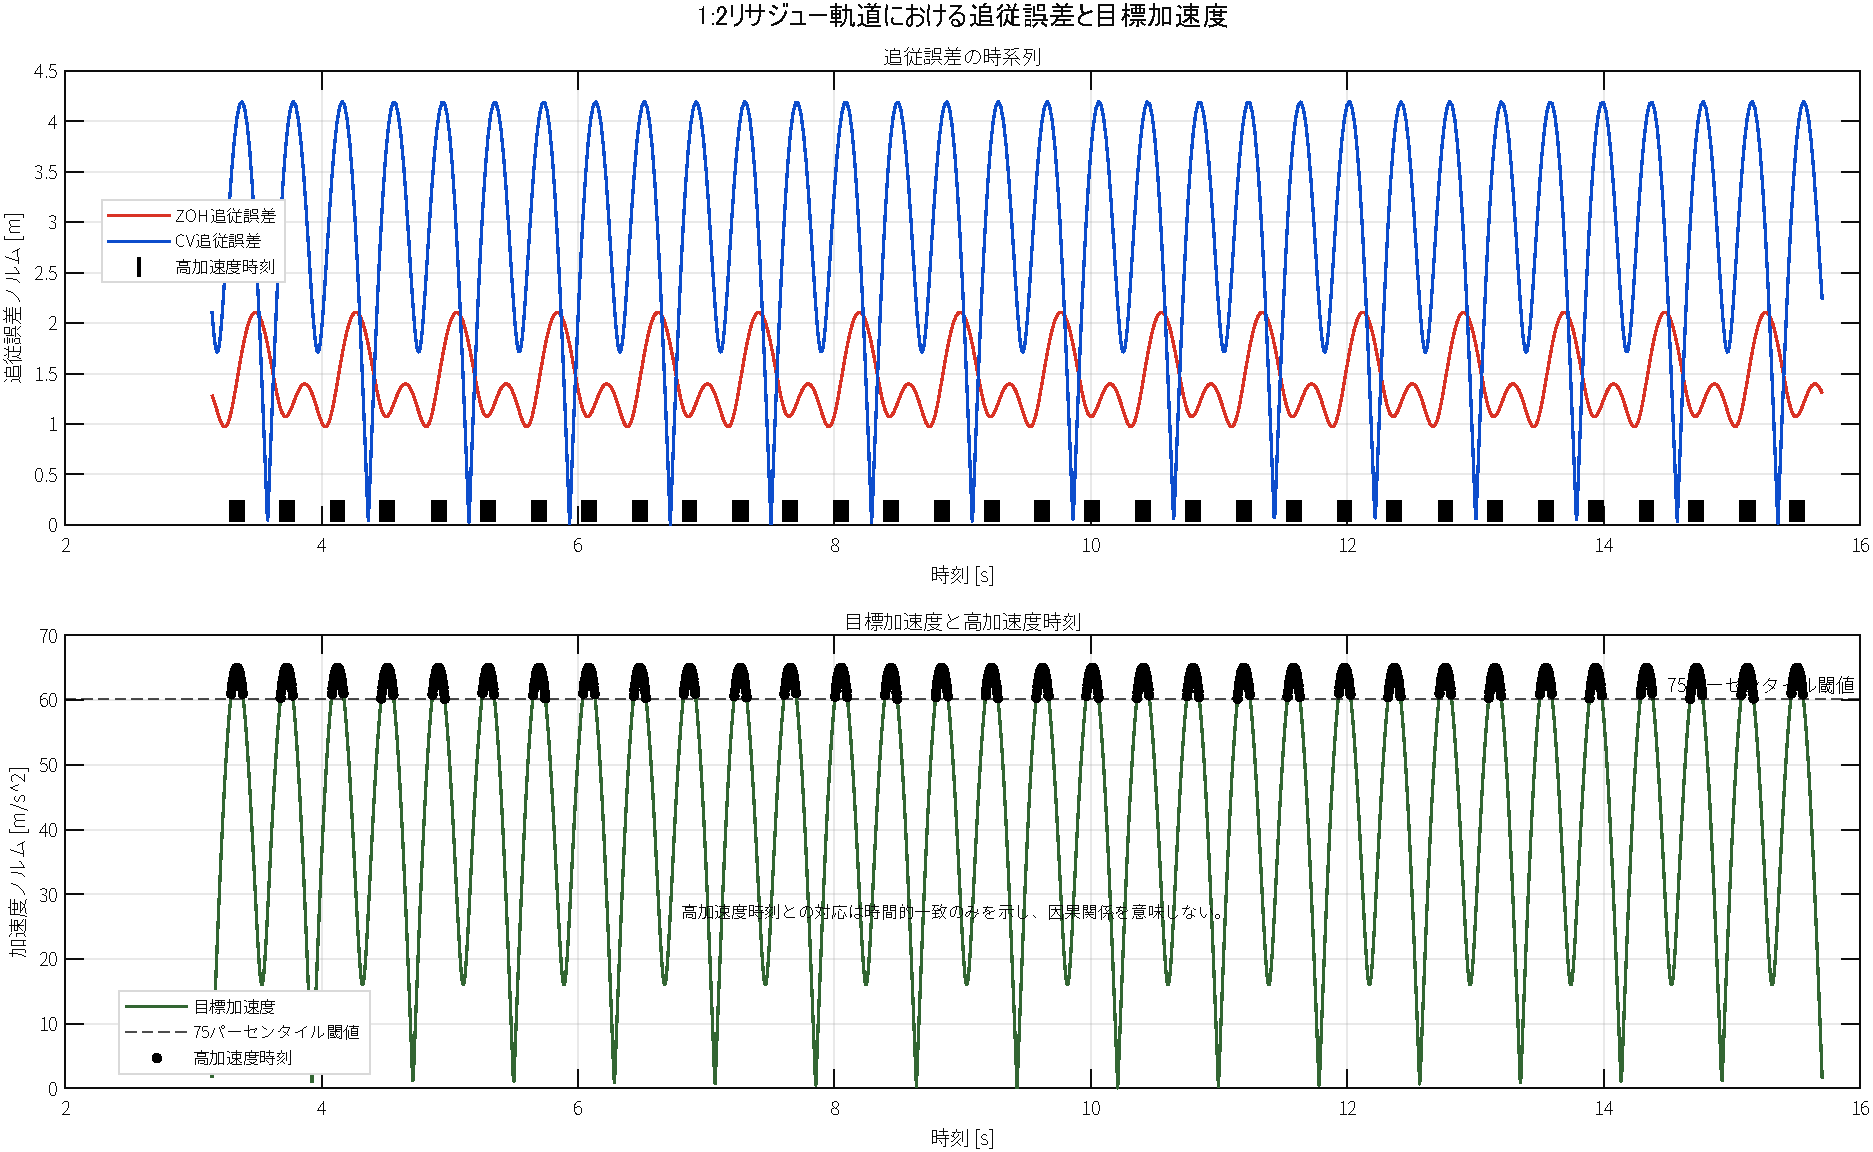
\includegraphics[width=\linewidth]{../assets/issue9/figures/figure_04_lissajous_error_timeseries.pdf}
\caption{1:2リサジュー軌道における追従誤差と目標加速度}
\label{fig:error}
\end{figure}

図\ref{fig:error}は、最大悪化条件 $\omega=4\ \mathrm{rad/s},\ L=0.5\ \mathrm{s}$ の追従誤差と目標加速度を示す。高加速度時刻は加速度ノルムの75パーセンタイル以上として表示した。CV誤差が周期的にZOH誤差を大きく上回る区間と高加速度時刻の時間的な対応が見られる。ただし、この図は時間的一致を示すものであり、高加速度だけが悪化の原因であることを証明するものではない。

\subsection{遅延・角周波数と性能比}

\begin{figure}[H]
\centering
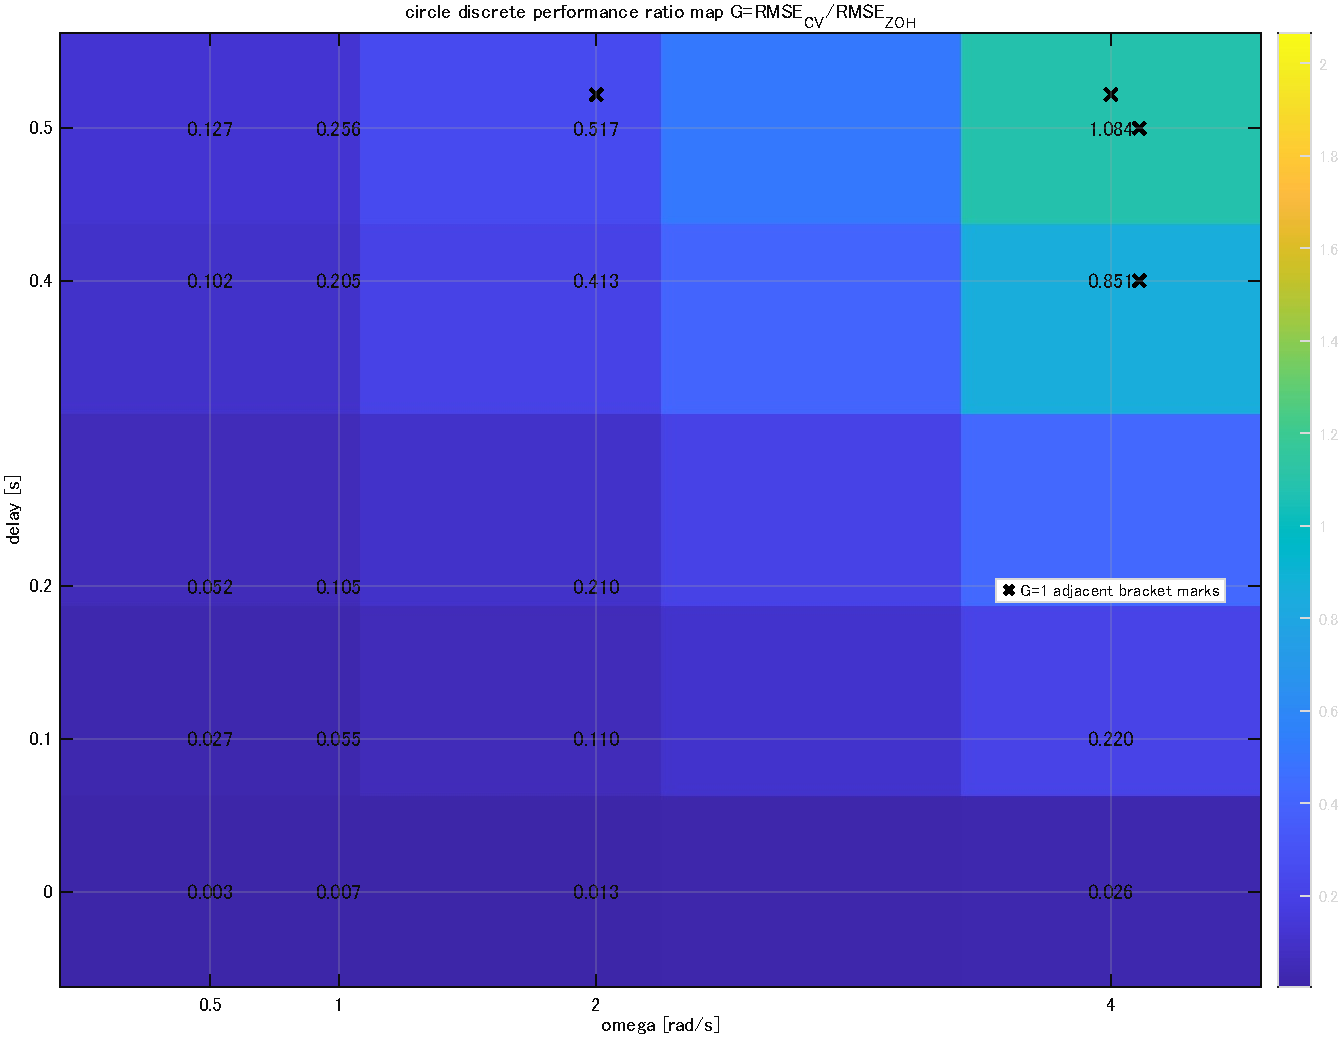
\includegraphics[width=0.96\linewidth]{../assets/issue9/figures/figure_05_circle_delay_omega_map.pdf}
\caption{円軌道における通信遅延・角周波数と性能比（$G<1$：CV優位）}
\label{fig:map-circle}
\end{figure}

\begin{figure}[H]
\centering
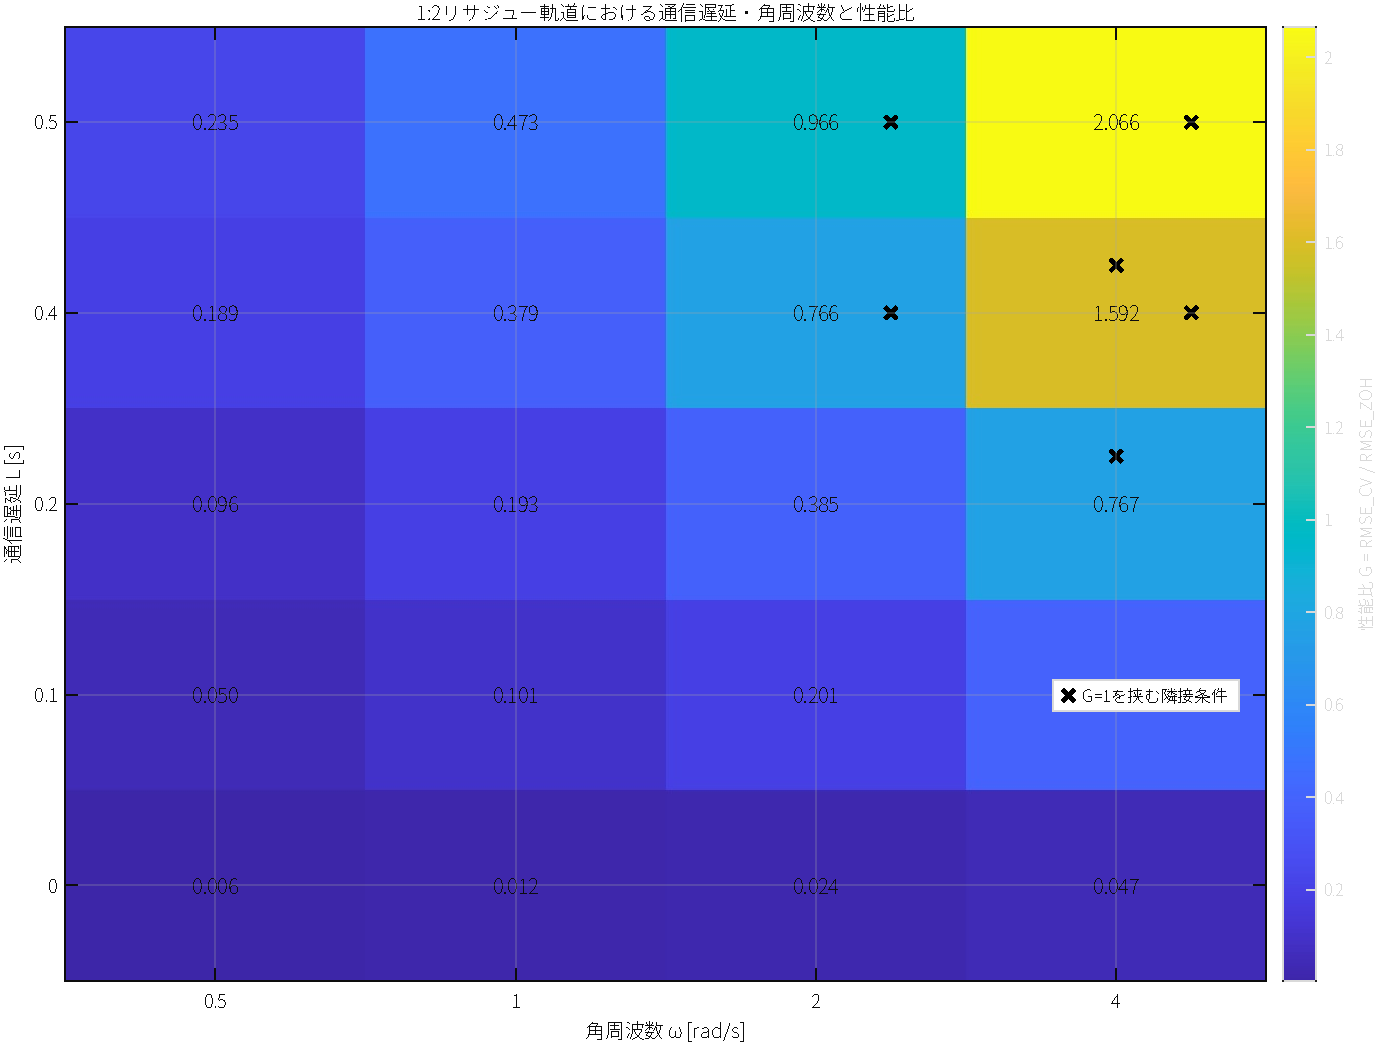
\includegraphics[width=0.96\linewidth]{../assets/issue9/figures/figure_06_lissajous_delay_omega_map.pdf}
\caption{1:2リサジュー軌道における通信遅延・角周波数と性能比（$G<1$：CV優位）}
\label{fig:map-liss}
\end{figure}

図\ref{fig:map-circle}、図\ref{fig:map-liss}では、遅延と角周波数の増加に伴って $G$ が大きくなる傾向が見られる。円軌道は $\omega=4\ \mathrm{rad/s},\ L=0.5\ \mathrm{s}$ で初めて悪化した。リサジュー軌道は同じ $\omega=4\ \mathrm{rad/s}$ でも $L=0.4\ \mathrm{s}$ から悪化し、円軌道よりCVの有効範囲が狭かった。

遅延がゼロでない条件でもCVは大きな改善を示した。例えば $\omega=2\ \mathrm{rad/s},\ L=0.2\ \mathrm{s}$ では、円軌道で $G=0.210$、1:2リサジュー軌道で $G=0.385$ であり、いずれもZOHよりRMSEが小さかった。

改善と悪化を挟む隣接格子および $G=1$ に最も近い隣接格子を表\ref{tab:boundary}に示す。本稿でいう「境界」は連続値として同定した点ではなく、探索した離散条件の中で改善側と悪化側を挟む隣接条件を意味する。条件間の補間は行っていない。同一の条件対が「改善--悪化」と「$G=1$最近傍」の複数の選定役割を兼ねる場合は、役割を明示するため重複して掲載した。

\begin{table}[H]
\centering
\caption{離散条件格子における性能境界の隣接条件}
\label{tab:boundary}
\scriptsize
\setlength{\tabcolsep}{2.7pt}
\begin{tabular}{lccccrrl}
\toprule
軌道 & 変化軸 & 固定条件 & 下側条件 & 上側条件 & 下側$G$ & 上側$G$ & 種別 \\
\midrule
円 & $L$ & $\omega=4$ & $L=0.4$ & $L=0.5$ & 0.851 & 1.084 & 改善--悪化 \\
円 & $\omega$ & $L=0.5$ & $\omega=2$ & $\omega=4$ & 0.517 & 1.084 & 改善--悪化 \\
円 & $L$ & $\omega=4$ & $L=0.4$ & $L=0.5$ & 0.851 & 1.084 & $G=1$最近傍 \\
1:2リサジュー & $L$ & $\omega=4$ & $L=0.2$ & $L=0.4$ & 0.767 & 1.592 & 改善--悪化 \\
1:2リサジュー & $\omega$ & $L=0.4$ & $\omega=2$ & $\omega=4$ & 0.766 & 1.592 & 改善--悪化 \\
1:2リサジュー & $\omega$ & $L=0.5$ & $\omega=2$ & $\omega=4$ & 0.966 & 2.066 & 改善--悪化 \\
1:2リサジュー & $L$ & $\omega=2$ & $L=0.4$ & $L=0.5$ & 0.766 & 0.966 & $G=1$最近傍 \\
\bottomrule
\end{tabular}
\end{table}

\subsection{無次元量による整理}

\begin{figure}[H]
\centering
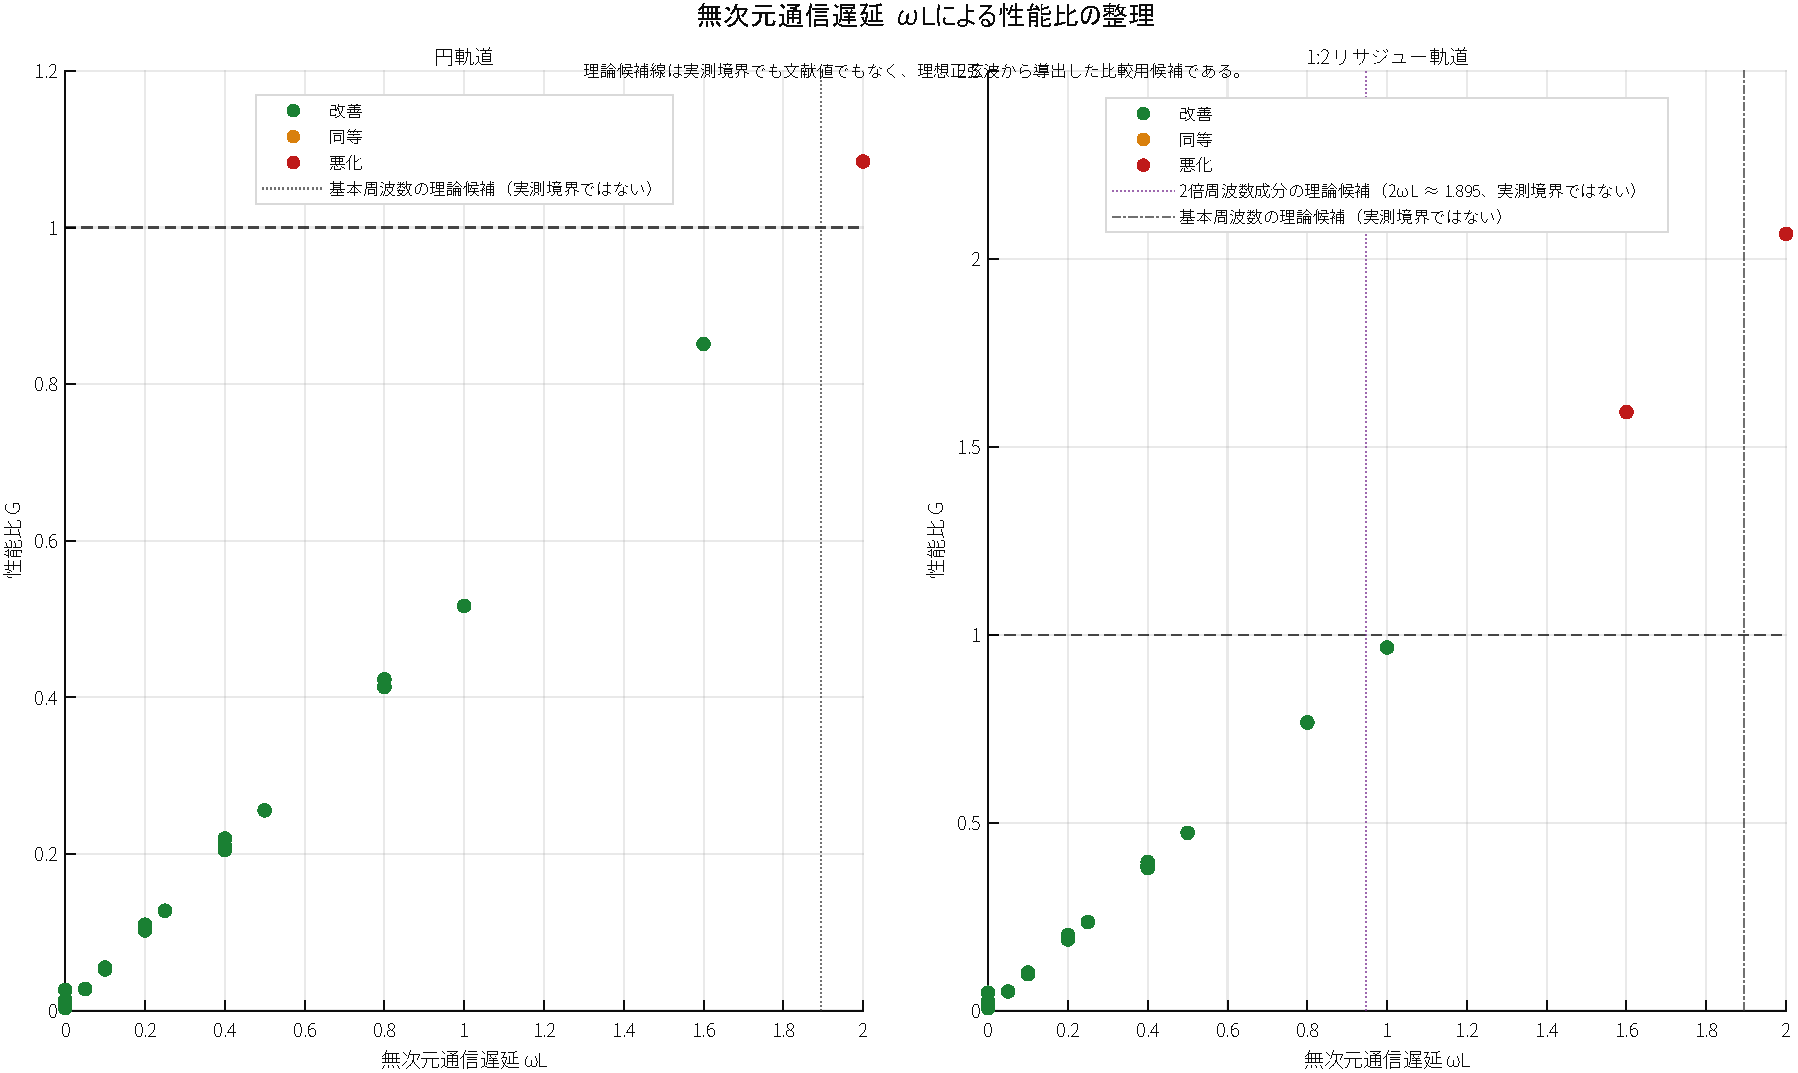
\includegraphics[width=\linewidth]{../assets/issue9/figures/figure_07_performance_vs_omega_delay.pdf}
\caption{無次元通信遅延 $\omega L$ による性能比の整理（$G<1$：CV優位）}
\label{fig:dimensionless-delay}
\end{figure}

\begin{figure}[H]
\centering
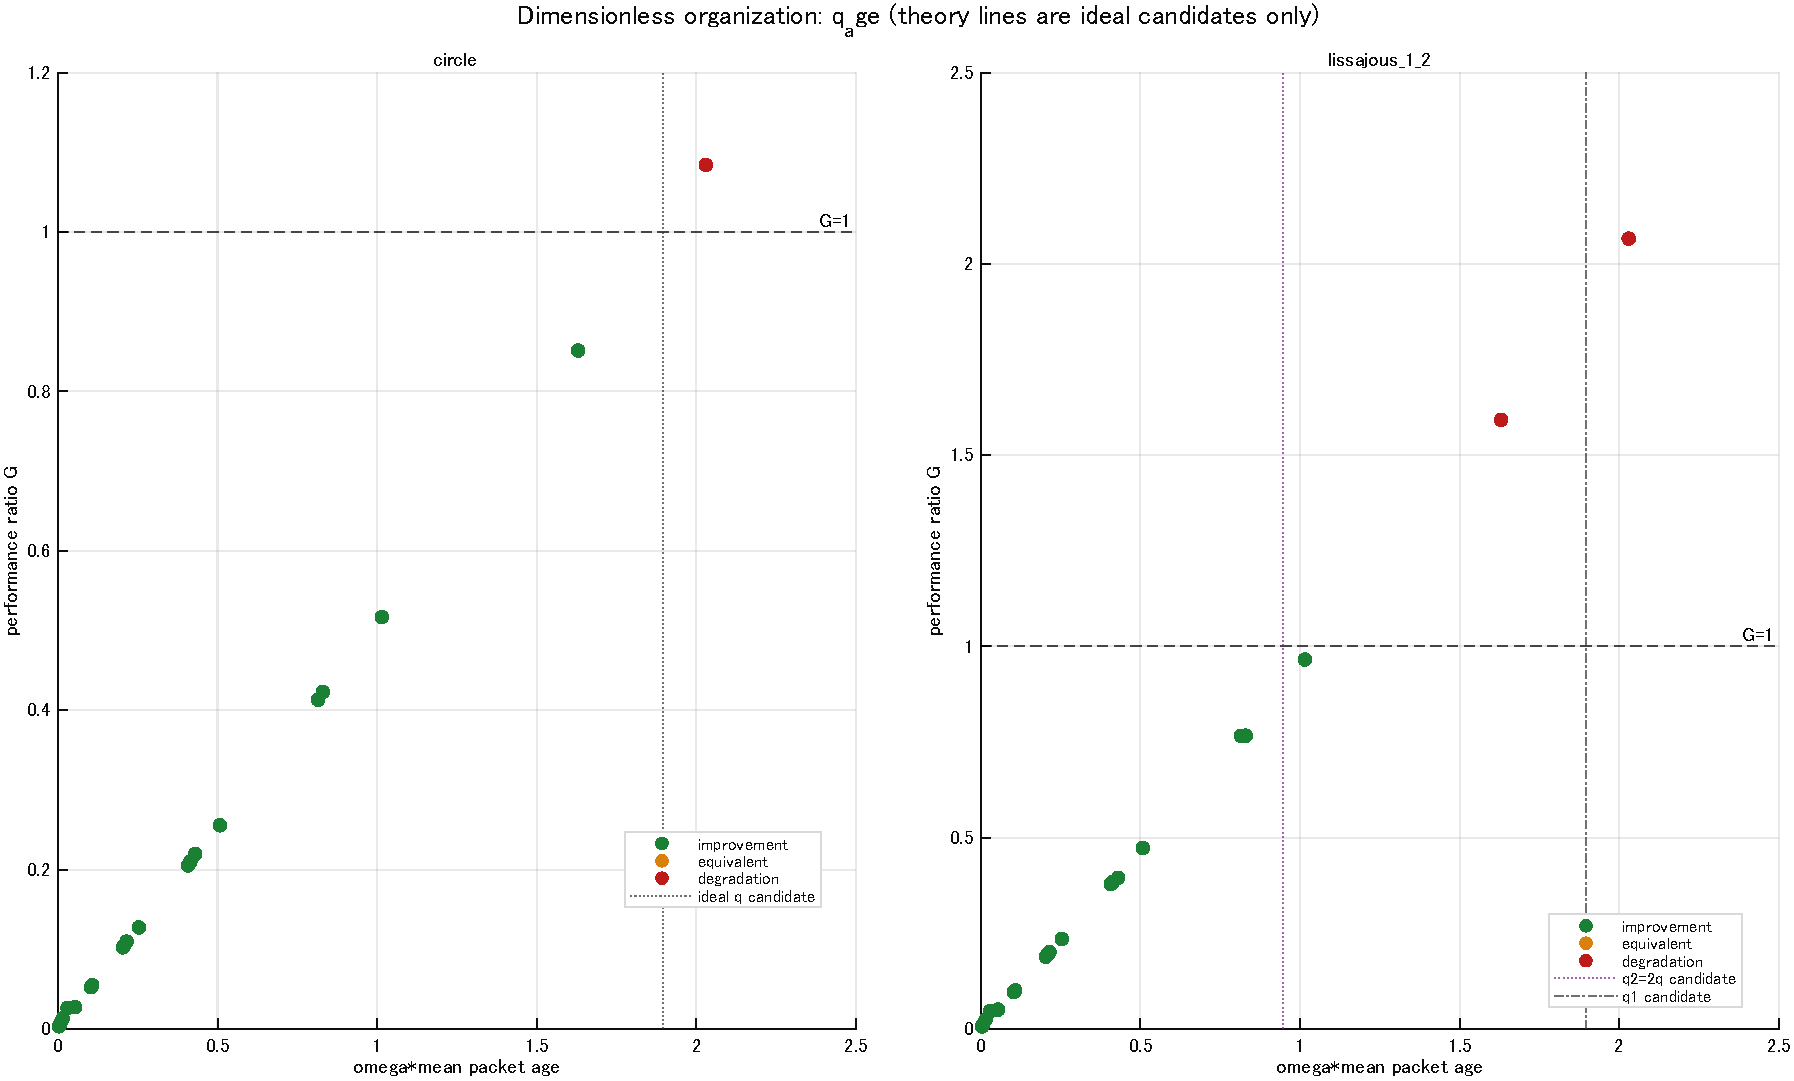
\includegraphics[width=\linewidth]{../assets/issue9/figures/figure_08_performance_vs_omega_mean_packet_age.pdf}
\caption{平均パケット齢に基づく無次元量による性能比の整理（$G<1$：CV優位）}
\label{fig:dimensionless-age}
\end{figure}

名目遅延が0であっても、送信周期が0.020 sであるため、評価区間の平均パケット齢は約0.0075 sであった。このためZOHにはサンプル間保持による誤差が残り、CVは $L=0$ の全条件でもRMSEを低減した。したがって、補償時間を名目遅延 $L$ だけでなく、実際に使用したパケットの齢で捉える必要がある。

円軌道の $\omega=4\ \mathrm{rad/s}$ では、$L=0.4$ と0.5 sの間で $G$ が0.851から1.084へ変化した。このとき $q_a=\omega\overline a$ は1.630から2.030であり、後述する理想正弦波の候補値1.895を挟んだ。リサジュー軌道では2倍周波数成分を含むため、単一の $\omega L$ または $\omega\overline a$ だけでは全条件を同じ境界で整理できなかった。

\subsection{数値収束}

代表5条件で時間刻みを半減した結果、最大 $|\Delta G|$ はリサジュー軌道の $\omega=4\ \mathrm{rad/s},\ L=0.5\ \mathrm{s}$ で0.0019707であった。円軌道の悪化条件では $G=1.0843$ から1.0853、リサジュー軌道の最大悪化条件では2.0661から2.0681となり、改善・悪化の分類は変化しなかった。したがって、主要な分類は少なくとも確認した代表条件では時間刻みによる見かけの反転ではない。

\section{考察}

\subsection{低遅延・低角周波数でCVが有効な理由}

目標位置を時刻 $t_k$ のまわりで Taylor 展開すると、
\begin{equation}
\vect r(t_k+a)=\vect r(t_k)+a\dot{\vect r}(t_k)
+\frac{a^2}{2}\ddot{\vect r}(t_k)+O(a^3)
\label{eq:taylor}
\end{equation}
となる。ZOHは第1項だけを使用するのに対し、CVは第2項までを再現する。そのため、パケット齢が短く、加速度が小さい条件では、ZOHに残る一次の位置遅れをCVが大きく低減する。40条件中37条件で改善したことは、この範囲では一次外挿の利益が高次の予測誤差を上回ったことを示す。

通信遅延 $L=0$ でもCVが改善した理由は、パケット齢が0ではないためである。ZOHは20 ms間隔のサンプル値を保持するが、CVはその間を速度情報によって前方外挿する。この結果は、サンプル値系では「通信遅延なし」と「常に最新の連続値を利用できること」が同義ではないことを示している。

ただし、最大改善率約99\%となった低速・遅延0の条件では、ZOHの絶対RMSE自体が円軌道で0.00458 m、リサジュー軌道で0.00722 mと小さい。相対改善率だけをもって実用上の効果が常に大きいと解釈してはならない。

\subsection{高角周波数・大遅延で悪化する理由}

式\eqref{eq:taylor}より、CVが無視する主要項は $a^2\ddot{\vect r}/2$ である。したがって、パケット齢が長いほど誤差は概ね二次的に増加し、角周波数が高く加速度や方向変化が大きいほど定速度仮定が崩れる。CVの外挿が正しい方向へ遅れを補う範囲を超えると、過去位置を保持するZOHより大きな誤差を生じる。

リサジュー軌道の最大悪化条件では、CVの最大誤差は4.194 m、ZOHは2.108 mであった。図\ref{fig:error}の高加速度時刻とCV誤差増大には時間的対応があるが、加速度、複数周波数成分、局所位置応答およびサンプリングが同時に作用しているため、高加速度だけを原因として断定することはできない。

\subsection{理想正弦波の境界候補}

理想的な単一正弦波に対し、パケット齢を一定と仮定して $q=\omega a$ とおく。以下の $E_{\mathrm{ZOH}}$ と $E_{\mathrm{CV}}$ は、まず受信側で再構成された位置指令の誤差振幅を表す。固定パケット齢、単一正弦波、定常状態という仮定では、両方式の誤差信号は同じ角周波数を持ち、共通の局所位置応答
\begin{equation}
\label{eq:local-frequency-response}
H(j\omega)=\frac{1}{1+j\omega T}
\end{equation}
を通過する。したがって、手先出力側の誤差振幅はそれぞれ $|H(j\omega)|E_{\mathrm{ZOH}}$ と $|H(j\omega)|E_{\mathrm{CV}}$ となり、両者が等しくなる条件では共通因子 $|H(j\omega)|$ が相殺される。このため、次の指令再構成誤差から求めた境界を、理想条件下では手先出力誤差の境界候補としても用いることができる。

振幅で正規化したZOHとCVの指令再構成誤差振幅の二乗は、
\begin{equation}
E_{\mathrm{ZOH}}^2=2(1-\cos q),
\qquad
E_{\mathrm{CV}}^2=(1-\cos q)^2+(q-\sin q)^2
\end{equation}
となる。両者が等しい非零の境界は
\begin{equation}
q=2\sin q
\end{equation}
を満たし、最初の正の非零解は $q\approx1.895494$ である。この値は文献から採用した境界ではなく、本課題の理想化モデルから導出した比較用候補である。

円軌道で観測された隣接条件は $q_a=1.630$ と2.030であり、候補値1.895はその間に入った。よって、今回の粗い離散格子では理想正弦波の予測と整合的である。ただし、境界を1.895と実測確定したわけではなく、正式に示せる範囲は隣接条件による1.630から2.030の間である。

\subsection{円軌道とリサジュー軌道の差}

円軌道は単一角周波数であり、速度の大きさが一定であるため、$q_a$による整理が比較的成立した。一方、1:2リサジュー軌道は $y$方向に $2\omega$ 成分を持ち、速度方向と加速度が周期的に大きく変化する。同じ $\omega=4\ \mathrm{rad/s},\ L=0.4\ \mathrm{s}$ でも、円軌道は $G=0.851$ で改善側、リサジュー軌道は $G=1.592$ で悪化側であった。

この比較から、少なくとも本モデルと設定した条件範囲では、CVの性能は通信遅延と基本角周波数だけでなく、周波数構成や方向変化を含む軌道の運動特性とも関係することが分かる。2倍周波数成分と大きな方向変化を含む1:2リサジュー軌道では、今回の条件範囲において円軌道より早い段階で悪化した。ただし、周波数成分、方向変化および加速度の寄与を個別に変化させていないため、各要因の寄与は分離できない。リサジュー軌道を単一の $q=\omega a$ だけで整理するのは不十分であり、2倍周波数成分については $2\omega a$ も考慮する必要がある。

\subsection{モデル化の限界}

本課題の結果には次の制約がある。
\begin{enumerate}[leftmargin=2.2em,itemsep=0.3em]
\item 人間操作者、映像フィードバックおよび双方向閉ループを含まない。
\item 局所位置応答を各軸独立の一次遅れに簡略化し、ロボットの運動学、飽和、接触および安全制約を含まない。
\item 速度は解析式から正確に与えており、実センサの雑音や速度推定誤差を含まない。
\item 遅延は一定で、パケット損失、遅延揺らぎおよび到着順序の入替えを含まない。
\item 軌道は円と1:2リサジューの2種類、遅延と角周波数は離散40条件に限られる。
\item 時定数 $T$ と送信周期 $h_s$ を固定したため、両者の独立効果を識別できない。
\item 理論候補 $q\approx1.895$ は、サンプリング、パケット齢変動、一次遅れの局所位置応答および複数周波数成分を無視した理想化結果である。
\end{enumerate}

したがって、本結果をそのまま実機遠隔操作の性能境界へ一般化することはできない。実システムへ適用するには、速度推定誤差、変動遅延、パケット損失、ロボット固有の動力学および人間の適応を追加して検証する必要がある。

\subsection{目的達成の判定}

本課題の目的は、CVがZOHより有効となる条件と悪化する条件を明らかにすることであった。40条件中37条件でCVが改善し、高角周波数・大遅延の3条件で悪化したことから、CVは広い範囲で有効であるが常に優れるわけではないことを確認した。円軌道では改善・悪化境界が理想正弦波の無次元候補と整合した。一方、2倍周波数成分と大きな方向変化を含む1:2リサジュー軌道では、今回の条件範囲において円軌道より早い段階で悪化した。ただし、各要因の寄与は個別に分離していない。

以上より、少なくとも本モデルと設定した条件範囲では、CVの性能は遅延時間単独ではなく、受信側で使用するパケット齢、軌道の運動時間スケール、および周波数構成や方向変化を含む運動特性と関係することが示された。

\section{結論}

遠隔地の操作者が生成する手先位置指令を片方向通信でロボット側へ送り、受信側でZOHまたはCVにより指令を再構成し、局所位置制御系を含むロボット手先が追従する状況をモデル化した。人間の入力は円軌道と1:2リサジュー軌道で代用し、固定サンプリング、固定通信遅延、最新パケット選択および一次遅れの局所位置応答を含む40条件を比較した。

CVは40条件中37条件でZOHよりRMSEを低減した。一方、高角周波数・大遅延では定速度仮定の誤差が増大し、円軌道の1条件とリサジュー軌道の2条件でZOHより悪化した。円軌道の境界近傍は $\omega\overline a=1.630$ から2.030の間にあり、理想正弦波から導出した候補 $q\approx1.895$ と整合した。2倍周波数成分と大きな方向変化を含む1:2リサジュー軌道では、今回の条件範囲において円軌道より早く悪化し、基本角周波数だけでは有効範囲を十分に整理できなかった。

したがって、少なくとも本モデルと設定した条件範囲では、定速度予測補償はパケット齢に対して目標軌道の変化が緩やかな場合に有効である一方、パケット齢や角周波数が大きく、高い周波数成分や大きな方向変化を含む運動では、外挿誤差によって悪化し得る。本課題では、その有効範囲を離散条件格子と無次元量によって定量的に示した。

\section{参考文献}

\begin{thebibliography}{9}
\small
\bibitem{sheridan1963}
T. B. Sheridan and W. R. Ferrell,
``Remote Manipulative Control with Transmission Delay,''
\textit{IEEE Transactions on Human Factors in Electronics},
vol. HFE-4, no. 1, pp. 25--29, 1963,
doi: 10.1109/THFE.1963.231283.

\bibitem{bejczy1990}
A. K. Bejczy, W. S. Kim, and S. C. Venema,
``The Phantom Robot: Predictive Displays for Teleoperation with Time Delay,''
in \textit{Proceedings of the IEEE International Conference on Robotics and Automation},
pp. 546--551, 1990,
doi: 10.1109/ROBOT.1990.126037.

\bibitem{zheng2018}
Y. Zheng, M. J. Brudnak, P. Jayakumar, J. L. Stein, and T. Ersal,
``A Predictor-Based Framework for Delay Compensation in Networked Closed-Loop Systems,''
\textit{IEEE/ASME Transactions on Mechatronics},
vol. 23, no. 5, pp. 2482--2493, 2018,
doi: 10.1109/TMECH.2018.2864722.

\bibitem{zheng2020}
Y. Zheng, M. J. Brudnak, P. Jayakumar, J. L. Stein, and T. Ersal,
``Evaluation of a Predictor-Based Framework in High-Speed Teleoperated Military UGVs,''
\textit{IEEE Transactions on Human-Machine Systems},
vol. 50, no. 6, pp. 561--572, 2020,
doi: 10.1109/THMS.2020.3018684.

\bibitem{zhang2023}
Q. Zhang, Z. Xu, Y. Wang, L. Yang, X. Song, and Z. Huang,
``Predicted Trajectory Guidance Control Framework of Teleoperated Ground Vehicles Compensating for Delays,''
\textit{IEEE Transactions on Vehicular Technology},
vol. 72, no. 9, pp. 11264--11274, 2023,
doi: 10.1109/TVT.2023.3269517.
\end{thebibliography}

\end{document}
